\documentclass[14pt]{extreport}
\usepackage{gost}



\begin{document}
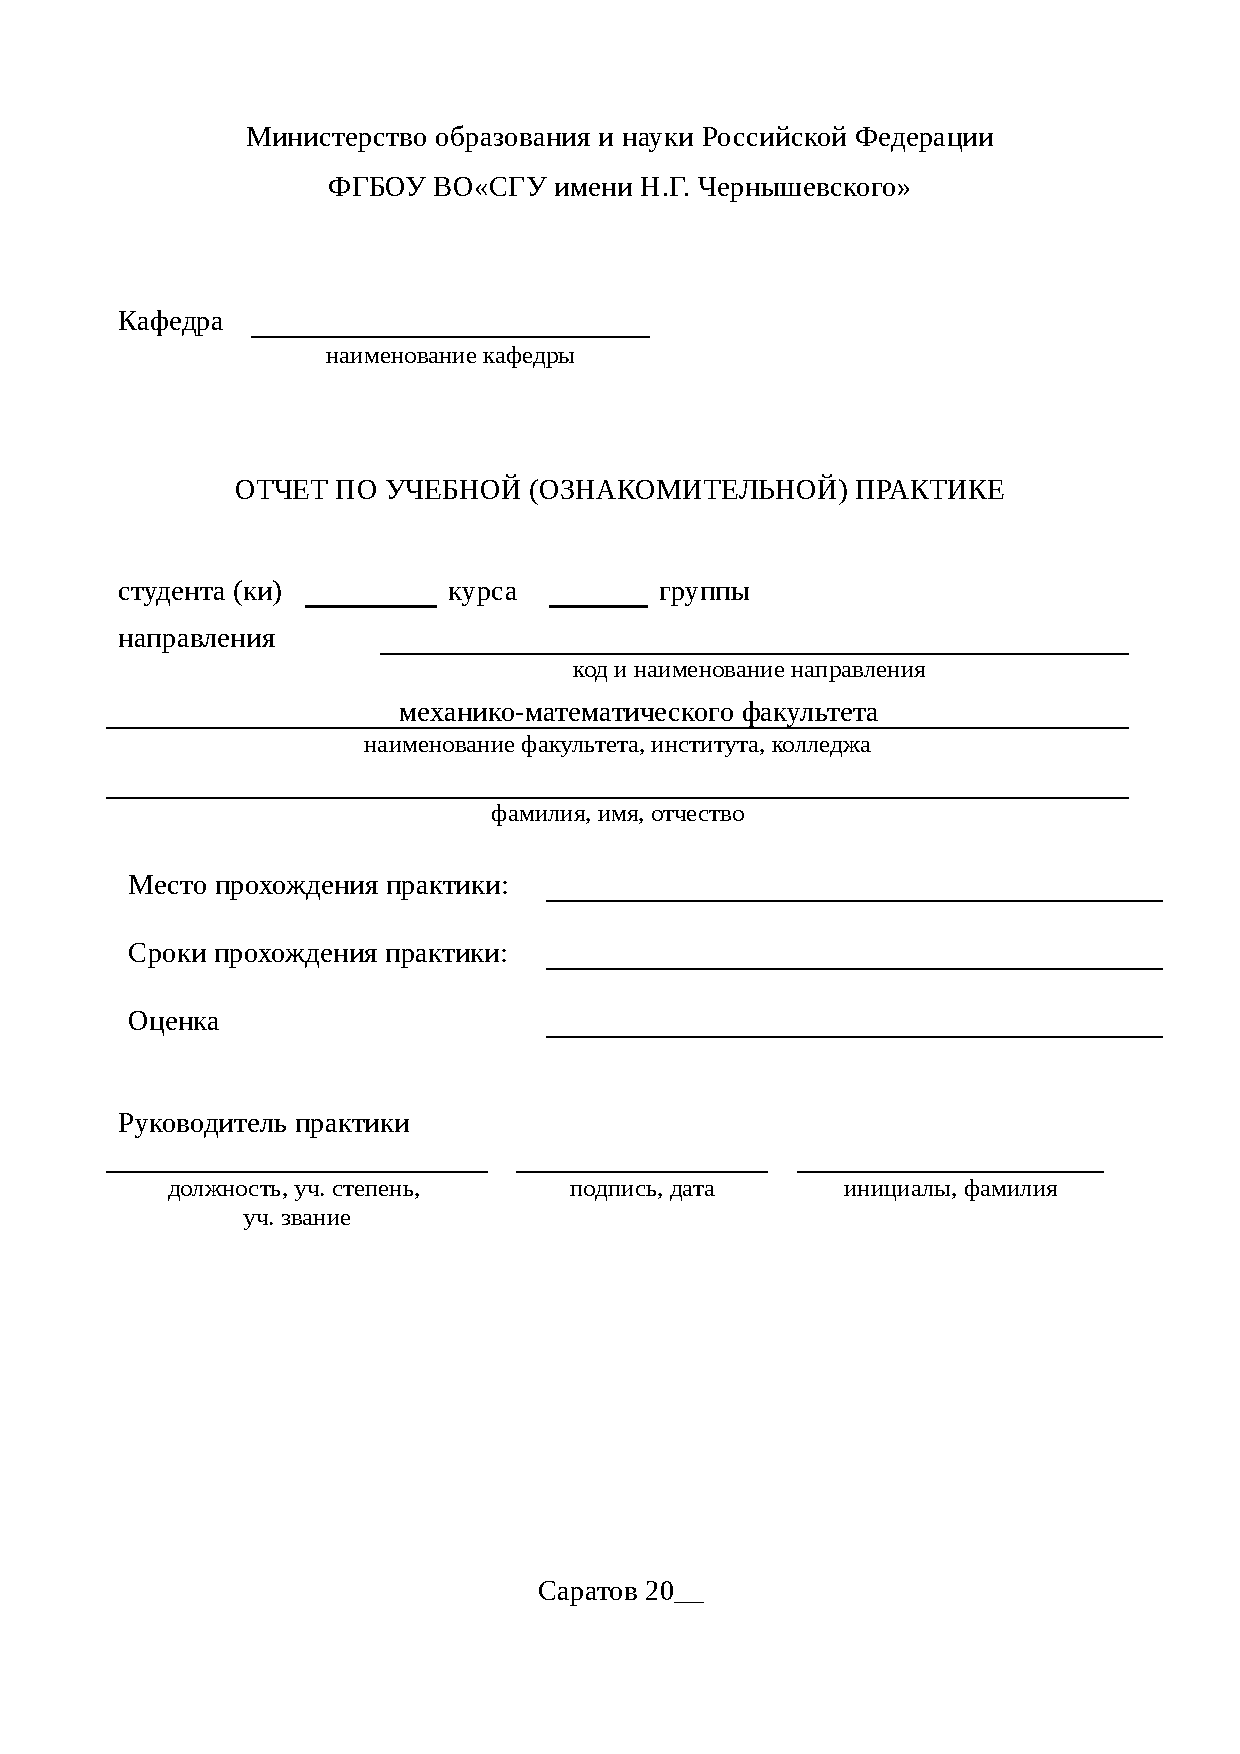
\includepdf[pages={1}]{titulOzPrac.pdf}


\tableofcontents

\intro

Ознакомительная практика является неотъемлемой частью учебного процесса. Студентам необходима подготовка к осознанному и углубленному изучению общепрофессиональных и специальных дисциплин и получение навыков самостоятельной практической работы по сбору фактического материала, составлению базы данных для различных исследований, анализа собранной информации.




\chapter{Множества. Действительные числа}

\section{Основные понятия}

Под множеством понимают совокупность (собрание, класс, семейство...) некоторых объектов, объединенных по какому-либо признаку.
Множество обозначается заглавными буквами, например $M$, $X$. Прописными латинскими буквами обозначаются элементы множеств, например $a$, $x$.
\begin{itemize}
\item $a \in M$ - элемент $a$ принадлежит множеству $M$;
\item $a \notin M$ - элемент $a$ не принадлежит множеству $M$;
\item $\exists$ - <<существует>>;
\item $\exists x \in M$ - существует $x$ из $M$;
\item $\forall$ - <<для любого>>, <<для всякого>>;
\item $a \wedge b$ - конъюнкция (<<и>>) - логическое умножение;
\item $a \vee b$  - дизъюнкция (<<или>>) - логическое сложение;
\item $\neg$ - <<не>> - логическое отрицание, например $\neg \forall x \in M$ - не для всех $x$ из $M$
\item $:$ - <<имеет место>>, <<такое что>>.
\end{itemize}



\section{Числовые множества. Множества действительных чисел}

Множества, элементами которых являются числа, называются \emph{числовыми}. Примерами числовых множеств являются:
\begin{itemize}
\item $N = \{1; 2; 3; ...; n; ...\}$ - множество натуральных чисел;
\item $Z_0 = \{0; 1; 2; ...; n; ...\}$ - множество целых неотрицательных чисел;
\item $Z = \{0; \pm 1; \pm 2; ...; \pm n; ...\}$ - множество целых чисел;
\item $Q = \{\frac mn : m \in Z, n \in N\}$ - множество рациональных чисел;
\item $R$ - множество действительных чисел.
\end{itemize} 

Действительные числа, не являющиеся рациональными, называются \emph{иррациональными}.



\section{Числовые промежутки. Окрестность точки}
\begin{example}
Пусть $x_0$ - любое дейтвительное число (точка на числовой прямой). \emph{Окрестностью} точки $x_0$ называется любой интервал $(a; b)$, содержащий точку $x_0$. В частности, интервал $(x_0 - \varepsilon, x_0 + \varepsilon)$, где $\varepsilon > 0$, называется $\varepsilon$-окрестностью точки $x_0$. Число $x_0$ называется \emph{центром}, а число $\varepsilon$ - \emph{радиусом}.

\begin{figure}[H]
\centerline{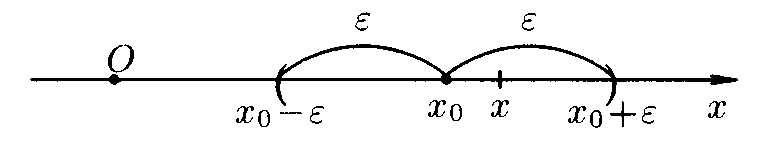
\includegraphics[width=1.0\linewidth]{pic1}}
\caption{Проверка точного решения}
\label{fig11}
\end{figure}

Если $x \in (x_0 - \varepsilon; x_0 + \varepsilon)$, то выполняется неравенство $x_0 - \varepsilon < x < x_0 + \varepsilon$, или, что то же, $|x - x_0| < \varepsilon$. Выполнение последнего неравенства означает попадание точки $x$ в $\varepsilon$-окрестность точки $x_0$ (см. рис. 1.1).
\end{example}





\chapter{Функция}


\section{Числовые функции. График функции}

\begin{example}
$f(x)=3x^2$
\begin{figure}[H]
\centerline{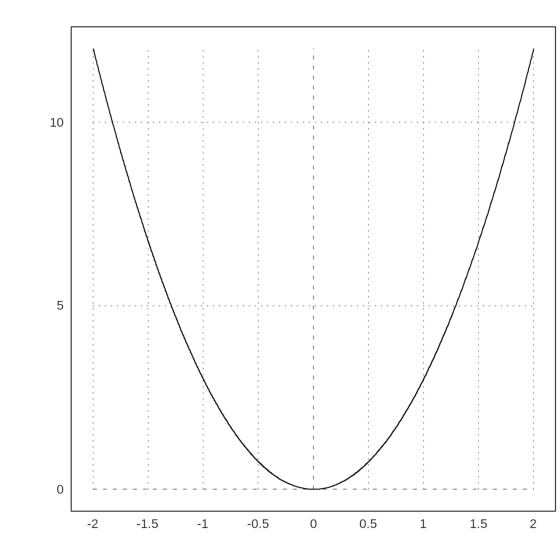
\includegraphics[width=1.0\linewidth]{gra-001}}
\caption{График функции - параболла}
\label{fig12}
\end{figure}
\end{example}

\begin{example}
$f(x)=|x|$
\begin{figure}[H]
\centerline{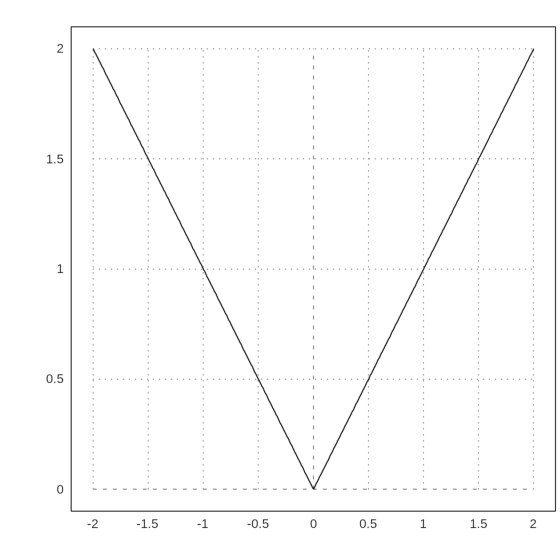
\includegraphics[width=1.0\linewidth]{gra-002}}
\caption{График функции - $f(x)=|x|$}
\label{fig13}
\end{figure}
\end{example}


\section{Обратная функция}
\begin{example}
Найти функцию обратную для $y=3x+2$

Выразим $x$ через $y$, получаем: 
\begin{equation}
x = \frac{1}{3}y-\frac{2}{3} 
\end{equation}

Это и есть обратная функция, переставив буквы $x$ и $y$, будем писать: $y=\frac{1}{3}x-\frac{2}{3}$.

Таким образом, $y=3x+2$ и $y=\frac{1}{3}x-\frac{2}{3}$ - взаимно обратные функции.
\begin{figure}[H]
\centerline{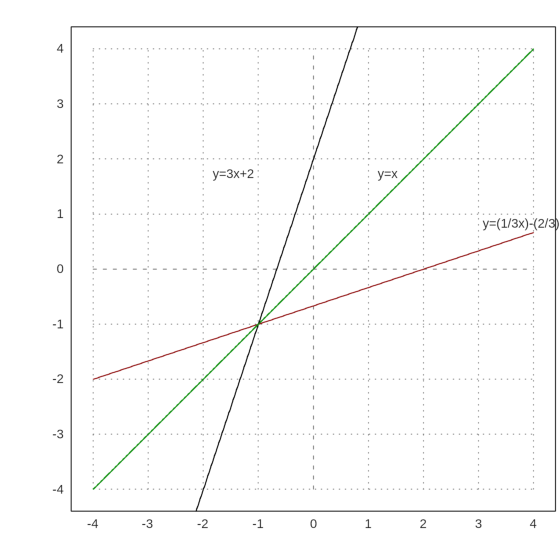
\includegraphics[width=1.0\linewidth]{gra-003}}
\caption{}
\label{fig14}
\end{figure}
\end{example}


\chapter{Последовательности}


\section{Предел числовой последовательности}
\begin{example}

Докажем, что:

$$\lim\limits_{n\to \infty}\frac{-1^n}{n}=0$$

Запишем определение предела: 
$$\forall \varepsilon<0 \exists n_0 = n(\varepsilon):\forall n \geqslant n_0 $$
$$\arrowvert\frac{-1^n}{n}-0\arrowvert<\varepsilon\Longrightarrow\frac{1}{n}<\varepsilon\Longrightarrow n(\varepsilon)>\frac{1}{\varepsilon}$$
$$n_0=[\frac{1}{\varepsilon}]+1$$
т.е. все члены последовательности начиная с такого $n_0$, лежат в интервале $(-\varepsilon; +\varepsilon)$.
\end{example}

\section{Предел монотонной ограниченной последовательности. Число $e$. Натуральные логарифмы}
\begin{theorem}
Последовательность с общим членом $e_n=(1+\frac{1}{n})^n$ имеет конечный предел при $n\rightarrow\infty$.
\end{theorem}
\begin{proof}

Покажем сначала, что $\{e_n\}$ представляет собой монотонно возрастающую последовательность. Согласно биному Ньютона, полагая $a=1, b=\frac{1}{n}$, получим

$$e_n=\left(1+\frac{1}{n}\right)^n=1+n\cdot\frac{1}{n}+\frac{n(n-1)}{2!}\cdot\frac{1}{n^2}+\frac{n(n-1)(n-2)}{3!}\cdot\frac{1}{n^3}+\dots+\frac{1}{n^n}=$$ $$=2+\frac{1}{2!}\left(1-\frac{1}{n}\right)+\frac{1}{3!}\left(1-\frac{1}{n}\right)\left(1-\frac{2}{n}\right)+\dots+\frac{1}{n!}\left(1-\frac{1}{n!}\right)\dots\left(1-\frac{n-1}{n}\right).$$

Аналогично,
$$e_n+1=\left(1+\frac{1}{n+1}\right)^N+1=2+\frac{1}{2!}\left(1-\frac{1}{n+1}\right)+\frac{1}{3!}\left(1-\frac{1}{n+1}\right)\left(1-\frac{2}{n+1}\right)+\dots$$

Далее докажем, что последовательность $\{e_n\}$ является ограниченной. Действительно, первый член любой монотонно возрастающей последовательности является ее наибольшей нижней границей и, таким образом, $e_n\geqslant 2$ для всех натуральных значений $n$. Перейдем к доказательству существования верхней границы. Очевидно, что
$$e_n=2+\frac{1}{2!}\left(1-\frac{1}{n}\right)+\frac{1}{3!}\left(1-\frac{1}{n}\right)\left(1-\frac{2}{n}\right)+\dots+\frac{1}{n!}\left(1-\frac{1}{n}\right)\dots\left(1-\frac{n-1}{n}\right)<$$ $$<2+\frac{1}{2!}+\frac{1}{3!}+\dots+\frac{1}{n!}.$$

Кроме того, $\frac{1}{k!}<\frac{1}{2^k}$ для всех $k>3$. Тогда
$$\frac{1}{4!}+\frac{1}{5!}+\dots+\frac{1}{n!}<\frac{1}{2^4}+\frac{1}{2^5}+\dots+\frac{1}{2^n}.$$

Правая часть этого неравенства представляет собой сумму членов убывающей геометрической прогрессии. В качестве верхней границы этой суммы выступает любое число $U\geqslant\frac{1}{8}.$ Таким образом, последовательность с общим членом
$$e_n=2+\frac{1}{2!}+\frac{1}{3!}+\dots+\frac{1}{n!}<2+\frac{1}{2}+\frac{1}{6}+\frac{1}{8}<3$$
представляет собой ограниченную монотонно возрастающую последовательностьи, следовательно, имеет конечный предел - согласно теореме о мнотонных последовательностях.

\end{proof}



\chapter{Предел функции}

\section{Предел функции в точке}
\begin{example}

На <<языке $\varepsilon - \delta,$>> или по Коши.

Используя $\varepsilon$ - $\delta$ - определение предела, показать что $\lim\limits_{x \to 3}(3x-2)=7.$

\emph{Решение.}
 Пусть $\varepsilon>0$ является произвольным положительным числом. Выберем $\delta=\frac{\varepsilon}{3}.$ Очевидно, что если 

$0<|x-3|<\delta,$

 то

$|f(x)-L|=|(3x-2)-7|=|3x-9|=3|x-3|<3\delta=3\cdot\frac{\varepsilon}{3}=\varepsilon.$

Данный предел доказан в соответствии с определением Коши.

\end{example}

\begin{example}
На <<языке последовательностей>>, или по Гейне.

Доказать, что $f(x)=\sin\frac{1}{x}$ не имеет предела в точке $0$.
$$\forall\{x_n'\}\rightarrow 0\exists\{x_n\} \rightarrow0$$
$$\{f(x_n')\}\rightarrow A_1\{f(x_n)\}\rightarrow A_2$$
$$x_n':\sin\frac{1}{x_n'}=0\Leftrightarrow\frac{1}{x_n'}=\pi n\Longrightarrow x_n'=\frac{1}{\pi n} \xrightarrow[n\neq 0]{n\rightarrow \infty}0$$
$$x_n'=\frac{1}{\pi n}\rightarrow0:f(x_n')=0\xrightarrow{n\neq0}0$$
$$x_n:\sin\frac{1}{x_n}=1\Leftrightarrow\frac{1}{x_n}=\frac{\pi}{2}+2\pi n \Longrightarrow x_n=\frac{1}{\frac{\pi}{2}+2\pi n}\xrightarrow[n\neq0]{n\rightarrow\infty}0$$
$$x_n=\frac{1}{\frac{\pi}{2}+2\pi n}\rightarrow0:f(x_n)=1\rightarrow1$$как считать пределы

Последовательность по Гейне не имеет предела.
\end{example}

\section{Односторонние пределы}

\begin{example}
Найти односторонние пределы функции $f(x)=\frac{1}{x}$ при $x\rightarrow0$

\emph{Решение.} Правый предел:
$$\lim\limits_{x\to 0+0}\frac{1}{x}=\lim\limits_{x\to 0+}\frac{1}{x}=f(0+0)=\frac{1}{0+0}=\frac{1}{0}=+\infty;$$

Левый предел: 
$$\lim\limits_{x\to 0-0}\frac{1}{x}=\lim\limits_{x\to 0-}\frac{1}{x}=f(0-0)=\frac{1}{0-0}=\frac{1}{-0}=-\infty.$$
\end{example}

\section{Предел функции при $x\to\infty$}

\begin{example}
Найти предел функции $f(x)=\frac{1}{x}$, при $x\rightarrow \infty$.

\emph{Решение.} Подставляем вместо $x$ бесконечность. Получаем, что последовательность значений функции является бесконечно малой величиной и поэтому имеет предел, равный нулю:
$$\lim\limits_{x\to \infty}\frac{1}{x}=\frac{1}{\infty}=0.$$

\end{example}


\section{Бесконечно большая функция}

Функция $y=f(x)$, заданная на всей числовой прямой, называется \emph{бесконечно большой при} $x\rightarrow \infty$, если для любого числа $M>0$ найдется такое число $N=N(M)>0$, что при всех $x$, удовлетворяющих неравенству $|x|>N$, выполняется неравенство $|f(x)|>M$. 
\begin{example}

a) Функция $f(x)=\frac{1}{x}$ - является бесконечно большой при $x\rightarrow 0$;

б) Функция $f(x)=x$ - является бесконечно большой при $x\rightarrow \infty$.

\end{example}



\chapter{Бесконечно малые функции}

Функция $y=f(x)$ называется \emph{бесконечно малой при} $x\rightarrow x_0$, если $$\lim\limits_{x\to x_0}f(x)=0.$$
\begin{example}
а) Функция $f(x)=x$ является бесконечно малой при $x\rightarrow 0$, поскольку ее предел в точке $a=0$ равен нулю. Согласно теореме о связи двустороннего предела с односторонними эта функция бесконечно малая как при $x\rightarrow+0$, так и при $x\rightarrow -0$;

б) Функция $f(x)=\frac{1}{x^2}$ - является бесконечно малой при $x\rightarrow \infty$ (а также при $x\rightarrow+\infty$ и при $x\rightarrow -\infty$.
\end{example}


\section{Связь между функцией, ее пределом и бесконечно малой функцией}
\begin{example}Доказать, что $\lim\limits_{x\to1}(x+5)=6$
\begin{proof}
Функцию $x+5$, стоящую под знаком предела, можно представить следующим образом:
$$x+5=6+(x-1)$$
где функция $\alpha(x)=x-1$ является бесконечно малой функцией при $x\rightarrow1$, поскольку 
$$\lim\limits_{x\to1}\alpha(x)=\lim\limits_{x\to1}(x-1)=0$$

Следовательно, согласно теореме о связи между функцией, ее пределом и бесконечно малой функцией, делаем вывод, что 
$$\lim\limits_{x\to 1}(x+5)=6$$

Что и требовалось доказать.

\end{proof}

\end{example}

\section{Основные теоремы о пределах}
\begin{example}
$\lim\limits_{x\to 10}13=13$
\end{example}

\begin{example}
$\lim\limits_{x\to 0}(x^2-3x+2)=\lim\limits_{x\to 0}x^2-\lim\limits_{x\to 0}3x+\lim\limits_{x\to 0}2=0^2-3\cdot0+2=2$	
\end{example}

\begin{example}
$\lim\limits_{x\to 0}(x^2\cdot \sin x)= \lim\limits_{x\to 0}x^2\cdot\lim\limits_{x \to 0}\sin x =0^2\cdot\sin 0=0$
\end{example}

\begin{example}
$\lim\limits_{x\to 1}2x^2=2\lim\limits_{x\to 1}x^2=2\cdot 1^2=2$
\end{example}

\begin{example}
$$\lim\limits_{x\to 2}\frac{x+1}{x^2-3}=\frac{\lim\limits_{x\to 2}(x+1)}{\lim\limits_{x\to 2}(x^2-3)}=\frac{2+1}{2^2-3}=\frac{3}{4-3}=\frac{3}{1}=3$$
\end{example}


\section{Первый замечательный предел}
\begin{example}
 $$\lim\limits_{x\to 0}\frac{\sin7x}{3x}=\frac{0}{0}=\lim\limits_{x\to 0}\frac{\sin7x}{3\cdot\frac{1}{7}\cdot7x}=\frac{1}{\frac{3}{7}}=\frac{7}{3}$$
\end{example}

\begin{example}
$$\lim\limits_{x\to 0}\frac{5x^2}{\sin^2\frac{x}{2}}=\frac{0}{0}=\lim\limits_{x\to 0}\frac{5x\cdot x}{\sin\frac{x}{2}\cdot\sin\frac{x}{2}}=\lim\limits_{x\to 0}\frac{5\cdot2\cdot2\cdot\frac{x}{2}\cdot\frac{x}{2}}{\sin\frac{x}{2}\cdot\sin\frac{x}{2}}=5\cdot2\cdot2=20$$
\end{example}


\section{Второй замечательный предел}
\begin{example}
$$\lim\limits_{x\to\infty}\left(\frac{x-2}{x+1}\right)^{2x+3}=\left(\frac{\infty}{\infty}\right)^\infty= \lim\limits_{x\to\infty}\left(\frac{x+1-3}{x+1}\right)^{2x+3}=\lim\limits_{x\to\infty}\left(1-\frac{3}{x+1}\right)^{2x+3}=$$ $$=\lim\limits_{x\to\infty}\left(1+\frac{1}{\frac{x+1}{-3}}\right)^{2x+3}=1^\infty=\lim\limits_{x\to\infty}\left(\left(1+\frac{1}{\frac{x+1}{-3}}\right)^{\frac{x+1}{-3}}\right)^{\frac{-3}{x+1}\cdot(2x+3)}=e^{-3\lim\limits_{x\to\infty}\frac{2x+3}{x+1}}=$$ $$=e^{\frac{\infty}{\infty}}=e^{-3\lim\limits_{x\to\infty}\frac{\frac{2x+3}{x}}{\frac{x+1}{x}}}=e^{-3\cdot2}=e^{-6}$$
\end{example}


\chapter{Эквивалентные бесконечно малые функции}
\section{Сравнение бесконечно малых функций}
\begin{example}
Являются ли функции $\alpha(x)=6(x^2-5x+6)$ и $\beta(x)=x^2-x-6$ эквивалентными бесконечно малыми при $x\rightarrow 3$.

\emph{Решение.} $$\lim\limits_{x\to3}\frac{\alpha(x)}{\beta(x)}=\lim\limits_{x\to3}\frac{5(x^2-5x+6)}{x^2-x-6}=\lim\limits_{x\to3}\frac{5(x-3)(x-2)}{(x-3)(x+2)}=\lim\limits_{x\to3}\frac{5(x-2)}{x+2}=\frac{5}{5}=1$$

Заданные функции $\alpha(x)=5(x^2-5x+6)$ и $\beta(x)=x^2-x-6$ являются эквивалентными бесконечно малыми.
\end{example}


\section{Эквивалентные беконечно малые и основные теоремы о них}
\begin{example}Найти предел $\lim\limits_{x\to0}\frac{3x+7x^2}{\sin2x}.$

\emph{Решение.} При $x\rightarrow0:\sin2x\sim2x$
$$\lim\limits_{x\to0}\frac{3x+7x^2}{\sin2x}=\lim\limits_{x\to0}\frac{x(3+7x)}{2x}=\lim\limits_{x\to0}\frac{3+7x}{2}=\frac{3}{2}$$
\end{example}


\begin{example}Найти предел $\lim\limits_{x\to0}\frac{5x-6x^3}{\tg3x}$

\emph{Решение}. При $x\rightarrow0:5x-6x^3\sim5x, \tg3x\sim3x$
$$\lim\limits_{x\to0}\frac{5x-6x^3}{\tg3x}\left[\frac{0}{0}\right]=\lim\limits_{x\to0}\frac{5x}{3x}=\lim\limits_{x\to0}\frac{5}{3}=\frac{5}{3}$$

\end{example}


\section{Применение эквивиалентных бесконечно малых функций}
\begin{example}Вычислить предел $\lim\limits_{x\to0}\frac{x^3-2x^2}{x^2+4x}$ 

\emph{Решение.} $$\lim\limits_{x\to0}\frac{x^3-2x^2}{x^2+4x}=\frac{0}{0}=\lim\limits_{x\to0}\frac{x^2(x-2)}{x(x-4)}=\lim\limits_{x\to0}\frac{x^{\rightarrow0}\cdot(x^{\rightarrow0}-2)}{x^{\rightarrow0}+4}=0$$
\end{example}


\chapter{Непрерывность функций}

\section{Непрерывность функции в точке}

\section{Непрерывность функции в интервале и на отрезке}

\section{Точки разрыва функции и их классификация}

\section{Основные теоремы о непрерывных функциях. Непрерывность элементарных функций}

\section{Свойства функций непрерывных на отрезке}



\chapter{Производная функции}


























\end{document}